%***********************************************************
% zewwww Slides Template
% Simon Reif & Benedikt Stelter, 31 January 2025
%
% Preamble
% This tex code is use to be run together with the
% corresponding Quarto file.
%***********************************************************

% Packages
\documentclass[11pt, aspectratio=169, t]{beamer}
\def\tightlist{}

\RequirePackage{beamerbaserequires}
\usepackage[style=apa]{biblatex}
\addbibresource{../references.bib}
\AtBeginBibliography{\footnotesize}

\usepackage[labelfont={color=black,bf}]{caption}
\usepackage{booktabs, longtable, colortbl, array}
\usepackage{threeparttable}
\usepackage{subcaption}

\usepackage[utf8]{inputenc}
\usepackage{graphicx, tikz, color,framed, xcolor}
\usetikzlibrary{decorations.pathreplacing,calc}

\usepackage{amsmath,amssymb, lmodern, array, multirow}
\usepackage{iftex}


% Use packages from YMAL header:
\usepackage{setspace}
\usepackage{bm}
\usepackage{lipsum}

\definecolor{zewwwwRed}{RGB}{139, 0, 0}
\definecolor{zewwwwGrey}{RGB}{167, 179, 205}

\setbeamercolor{itemize item}{fg=zewwwwGrey}
\setbeamercolor{itemize subitem}{fg=zewwwwGrey}
\setbeamercolor{itemize subsubitem}{fg=zewwwwGrey}

\captionsetup[figure]{labelformat=empty, font=bf}% redefines the caption setup of the figures environment in the beamer class.
\captionsetup[table]{labelformat=empty, font=bf}% redefines the caption setup of the tables environment in the beamer class.

\setbeamertemplate{itemize item}[square]
\setbeamertemplate{itemize subitem}[circle]
\setbeamertemplate{itemize subsubitem}[circle]
\setbeamertemplate{frametitle continuation}{}

\setbeamercolor{bibliography item}{fg=black}
\setbeamercolor{bibliography entry author}{fg=black}
\setbeamercolor{bibliography entry title}{fg=black}
\setbeamercolor{bibliography entry location}{fg=black}
\setbeamercolor{bibliography entry note}{fg=black}
\setbeamertemplate{bibliography item}{}

\setbeamertemplate{blocks}[rounded][shadow=false]
\addtobeamertemplate{block begin}{\pgfsetfillopacity{0.8}}{\pgfsetfillopacity{1}}
\setbeamercolor{structure}{fg=zewwwwRed}
\setbeamercolor*{block title example}{fg=white,
bg= zewwwwRed}
\setbeamercolor*{block body example}{fg= black,
bg= zewwwwGrey!30}

% Allow shaded environment for code display
\usepackage{color}
\usepackage{fancyvrb}
\newcommand{\VerbBar}{|}
\newcommand{\VERB}{\Verb[commandchars=\\\{\}]}
\DefineVerbatimEnvironment{Highlighting}{Verbatim}{commandchars=\\\{\}}
% Add ',fontsize=\small' for more characters per line
\usepackage{framed}
\definecolor{shadecolor}{RGB}{241,243,245}
\newenvironment{Shaded}{\begin{snugshade}}{\end{snugshade}}
\newcommand{\AlertTok}[1]{\textcolor[rgb]{0.68,0.00,0.00}{#1}}
\newcommand{\AnnotationTok}[1]{\textcolor[rgb]{0.37,0.37,0.37}{#1}}
\newcommand{\AttributeTok}[1]{\textcolor[rgb]{0.40,0.45,0.13}{#1}}
\newcommand{\BaseNTok}[1]{\textcolor[rgb]{0.68,0.00,0.00}{#1}}
\newcommand{\BuiltInTok}[1]{\textcolor[rgb]{0.00,0.23,0.31}{#1}}
\newcommand{\CharTok}[1]{\textcolor[rgb]{0.13,0.47,0.30}{#1}}
\newcommand{\CommentTok}[1]{\textcolor[rgb]{0.37,0.37,0.37}{#1}}
\newcommand{\CommentVarTok}[1]{\textcolor[rgb]{0.37,0.37,0.37}{\textit{#1}}}
\newcommand{\ConstantTok}[1]{\textcolor[rgb]{0.56,0.35,0.01}{#1}}
\newcommand{\ControlFlowTok}[1]{\textcolor[rgb]{0.00,0.23,0.31}{\textbf{#1}}}
\newcommand{\DataTypeTok}[1]{\textcolor[rgb]{0.68,0.00,0.00}{#1}}
\newcommand{\DecValTok}[1]{\textcolor[rgb]{0.68,0.00,0.00}{#1}}
\newcommand{\DocumentationTok}[1]{\textcolor[rgb]{0.37,0.37,0.37}{\textit{#1}}}
\newcommand{\ErrorTok}[1]{\textcolor[rgb]{0.68,0.00,0.00}{#1}}
\newcommand{\ExtensionTok}[1]{\textcolor[rgb]{0.00,0.23,0.31}{#1}}
\newcommand{\FloatTok}[1]{\textcolor[rgb]{0.68,0.00,0.00}{#1}}
\newcommand{\FunctionTok}[1]{\textcolor[rgb]{0.28,0.35,0.67}{#1}}
\newcommand{\ImportTok}[1]{\textcolor[rgb]{0.00,0.46,0.62}{#1}}
\newcommand{\InformationTok}[1]{\textcolor[rgb]{0.37,0.37,0.37}{#1}}
\newcommand{\KeywordTok}[1]{\textcolor[rgb]{0.00,0.23,0.31}{\textbf{#1}}}
\newcommand{\NormalTok}[1]{\textcolor[rgb]{0.00,0.23,0.31}{#1}}
\newcommand{\OperatorTok}[1]{\textcolor[rgb]{0.37,0.37,0.37}{#1}}
\newcommand{\OtherTok}[1]{\textcolor[rgb]{0.00,0.23,0.31}{#1}}
\newcommand{\PreprocessorTok}[1]{\textcolor[rgb]{0.68,0.00,0.00}{#1}}
\newcommand{\RegionMarkerTok}[1]{\textcolor[rgb]{0.00,0.23,0.31}{#1}}
\newcommand{\SpecialCharTok}[1]{\textcolor[rgb]{0.37,0.37,0.37}{#1}}
\newcommand{\SpecialStringTok}[1]{\textcolor[rgb]{0.13,0.47,0.30}{#1}}
\newcommand{\StringTok}[1]{\textcolor[rgb]{0.13,0.47,0.30}{#1}}
\newcommand{\VariableTok}[1]{\textcolor[rgb]{0.07,0.07,0.07}{#1}}
\newcommand{\VerbatimStringTok}[1]{\textcolor[rgb]{0.13,0.47,0.30}{#1}}
\newcommand{\WarningTok}[1]{\textcolor[rgb]{0.37,0.37,0.37}{\textit{#1}}}

% Add new pandocbounced command to comply with pandoc update 3.5
\makeatletter
\newsavebox\pandoc@box
\newcommand*\pandocbounded[1]{% scales image to fit in text height/width
  \sbox\pandoc@box{#1}%
  \Gscale@div\@tempa{\textheight}{\dimexpr\ht\pandoc@box+\dp\pandoc@box\relax}%
  \Gscale@div\@tempb{\linewidth}{\wd\pandoc@box}%
  \ifdim\@tempb\p@<\@tempa\p@\let\@tempa\@tempb\fi% select the smaller of both
  \ifdim\@tempa\p@<\p@\scalebox{\@tempa}{\usebox\pandoc@box}%
  \else\usebox{\pandoc@box}%
  \fi%
}
\makeatother

% Make font size of minipage scriptsize by default s.t. table notes are small
\AtBeginEnvironment{minipage}{\scriptsize}

% Insert invers color Section Title Slide
\AtBeginSection{
\addtocounter{framenumber}{0} %Ignore Black Headline Pages for slide count
\usebackgroundtemplate{
\includegraphics[width=\paperwidth,height=\paperheight]{zewwwwImages/bg.png}}
\begin{frame}[c, noframenumbering, plain]
\begin{minipage}{300pt}
\textcolor{white}{\huge\secname}
\end{minipage}
\end{frame}

\usebackgroundtemplate{
\includegraphics[width=\paperwidth,height=\paperheight]{zewwwwImages/bgmain.pdf}}

\setbeamertemplate{footline}{%
\raisebox{10pt}{\makebox[\paperwidth]{\hfill{\tiny Simon \textcolor{zewwwwRed}{\bfseries{|}} \insertframenumber \makebox[10pt]{} }}}}
}

\makeatletter
\patchcmd\beamer@@tmpl@frametitle{sep=0.8cm}{sep=2cm}{}{}
\makeatother

\beamertemplatenavigationsymbolsempty
\setbeamertemplate{frametitle}{\textcolor{black}{\insertframetitle}}
\addtobeamertemplate{frametitle}{\vskip3ex}{}
\providecommand{\tightlist}{%
	\setlength{\itemsep}{0pt}\setlength{\parskip}{0pt}}

\begin{document}
% Title page
{
\addtocounter{framenumber}{-1} %Ignore Titlepage for slide count
\usebackgroundtemplate{
\includegraphics[width=\paperwidth,height=\paperheight]{zewwwwImages/bgtitle.png}}
\begin{frame}[c]

\begin{tikzpicture}[remember picture,overlay]
  \node[anchor=south west,inner sep=0pt] at (-0.2,2.5) {
   
\includegraphics[height=0.7cm]{zewwwwImages/yourlogo.png}
  };
  \node[anchor=south west,inner sep=0pt] at (-0.2,1.8) {
   
\includegraphics[height=0.7cm]{zewwwwImages/empty.png}
  };
\end{tikzpicture}
\begin{tikzpicture}
\node[overlay, anchor=south west, align=left, text width=0.54\linewidth] at (-0.4,-1.2) {\baselineskip=16pt\textcolor{white}{\textbf{\Large Introducing
the zewwwwEcon Presentation Template}} \par};
\node[overlay, anchor=north west, align=left, text width=9.8cm] at (-0.4,-1.2) { 	\textcolor{white}{Lord
Macbeth} \textcolor{zewwwwGrey}{\bfseries{|}}	\textcolor{white}{Thane of
Glamis} \\
		\textcolor{white}{Lady
Macbeth} \textcolor{zewwwwGrey}{\bfseries{|}}	\textcolor{white}{Queen of
Scotland} \\
	 \vspace{10pt} \textcolor{white}{\textbf{Dunsinane
Hill}} \textcolor{zewwwwGrey}{\bfseries{|}} \textbf{\textcolor{white}{10
Jun 2025}}}
;
\end{tikzpicture}
\end{frame}
}

% Main page
\setbeamertemplate{footline}{%
  \raisebox{10pt}{\makebox[\paperwidth]{\hfill{\tiny Simon \textcolor{zewwwwRed}{\bfseries{|}} \insertframenumber \makebox[10pt]{} }}}}

% Define background
\usebackgroundtemplate{
\includegraphics[width=\paperwidth,height=\paperheight]{zewwwwImages/bgmain.pdf}}

\begin{frame}{Introduction}
\phantomsection\label{introduction}
This Quarto template is supposed to make writing and presenting economic
research easy. Since everything from data to publication is happening in
the same environment, everything is easily reproducible and output can
be modified for the paper and the presentation at the same time.

You can for example

\begin{itemize}
\tightlist
\item
  Displaying text in different forms
\item
  Handling images
\item
  Graphs that fit the aesthetic of the slides
\item
  Tables 1 to 3 of a standard econ project
\end{itemize}
\end{frame}

\section{The various forms of displaying text in a
presentation}\label{the-various-forms-of-displaying-text-in-a-presentation}

\begin{frame}{Different text inputs}
\phantomsection\label{different-text-inputs}
You can make bullet lists with different levels

\begin{itemize}
\tightlist
\item
  This looks nice and helps separate thoughts
\item
  But you should always have two bullets, otherwise it looks a bit
  weired

  \begin{itemize}
  \tightlist
  \item
    Which to be fair one can argue about

    \begin{itemize}
    \tightlist
    \item
      At least on the third level
    \end{itemize}
  \end{itemize}
\item
  And going back to the first level
\end{itemize}

Sometimes one might need equations. Just use \LaTeX~for this in the text
to show that \(2^{2} > 3\). You can also have your equation stand out
like this:

\[\hat{\beta} = (X'X)^{-1} X'Y\]
\end{frame}

\begin{frame}{Text and picture side by side using columns}
\phantomsection\label{text-and-picture-side-by-side-using-columns}
There is a very small (0.4\%) column on the left that aligns the first
context column with the headline. These type of slides are in general
not much fun to produce.

\begin{columns}[T]
\begin{column}{0.004\linewidth}
\end{column}

\begin{column}{0.446\linewidth}
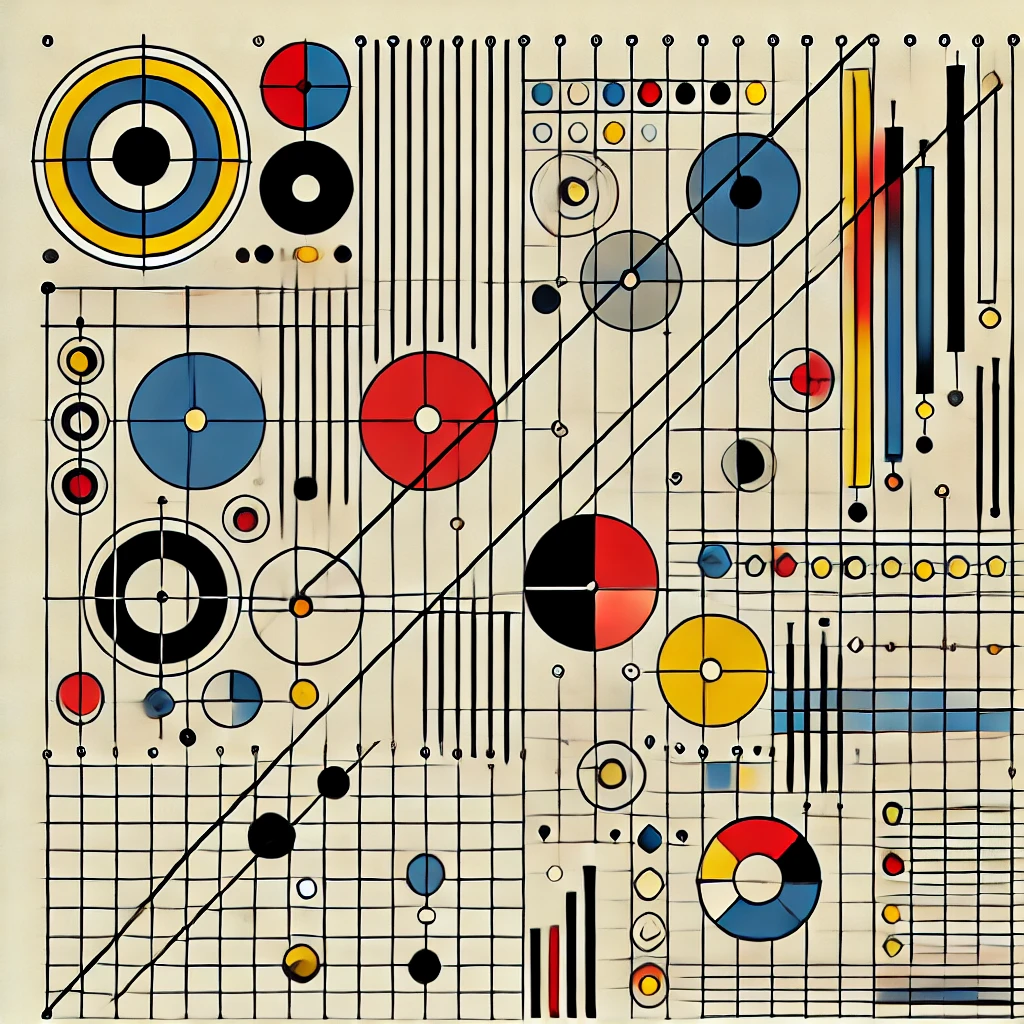
\includegraphics[width=\linewidth,height=1.80556in,keepaspectratio]{pictures/OLSpic.png}
\newline \scriptsize\textbf{Source:} Dall-E drawing a Bauhaus style
representation of the OLS mechanism.
\end{column}

\begin{column}{0.55\linewidth}
\normalsize

\begin{equation}
\frac{\partial S(\beta)}{\partial \beta} = -2X^\top (y - X\beta) = 0
\end{equation}

\begin{equation}
X^\top X \hat{\beta} = X^\top y
\end{equation}

\begin{equation}
\hat{\bm{\beta}} = (X^\top X)^{-1} X^\top y
\end{equation}

These equations minimize the sum of squared residuals \(S\). While this
seems promising, others argue that this has been done before. It is even
used to health insurance risk adjustment
\autocite[EJHE]{reifSettingIncentivesRight2025}.
\end{column}
\end{columns}
\end{frame}

\begin{frame}{Highlighting and References}
\phantomsection\label{highlighting-and-references}
Sometimes it seems that not only are people putting books from boxes but
also like boxes around some highlight text. An example would be
something you (can not) find in
\textcite[EJHE]{reifSettingIncentivesRight2025}:

\begin{exampleblock}{Defining an example}
\normalsize A lot could be in here. A definition. An equation.  A reference to \textcite[EJHE]{reifSettingIncentivesRight2025}. Not that since this is pure \LaTeX, you need to also use the respective cite styles \autocites[EJHE]{reifSettingIncentivesRight2025}. 
\end{exampleblock}
\end{frame}

\begin{frame}[fragile]{Show code and Output}
\phantomsection\label{show-code-and-output}
\begin{Shaded}
\begin{Highlighting}[]
\CommentTok{\# We can use code that is displayed in the output}
\DecValTok{2}\SpecialCharTok{\^{}}\DecValTok{2}
\end{Highlighting}
\end{Shaded}

\begin{verbatim}
[1] 4
\end{verbatim}

\begin{Shaded}
\begin{Highlighting}[]
\DecValTok{2}\SpecialCharTok{\^{}}\DecValTok{2} \SpecialCharTok{\textgreater{}} \DecValTok{3}
\end{Highlighting}
\end{Shaded}

\begin{verbatim}
[1] TRUE
\end{verbatim}
\end{frame}

\section{Graphs}\label{graphs}

\begin{frame}{Histogram}
\phantomsection\label{histogram}
\begin{figure}

\caption{\label{fig-hist}Distribution of height (in cm) in random data}

\centering{

\pandocbounded{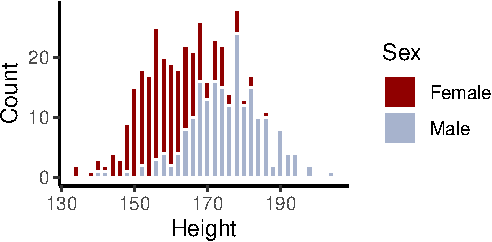
\includegraphics[keepaspectratio]{example_slides_files/figure-beamer/Histogram-1.pdf}}

\vspace{-5pt}
\begin{minipage}{0.9\textwidth}
\scriptsize
\singlespacing
\textbf{Notes:} You can use this text to provide further information about the table. \lipsum[66]
\end{minipage}
\vspace{15pt}

}

\end{figure}%
\end{frame}

\begin{frame}{Barchart}
\phantomsection\label{barchart}
\begin{figure}

\caption{\label{fig-barchart}Number of Federal States by Country}

\centering{

\pandocbounded{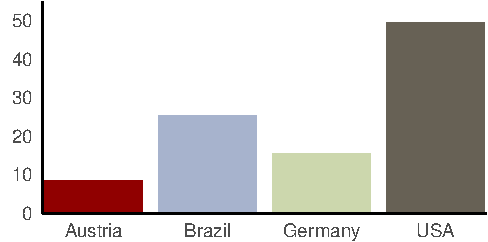
\includegraphics[keepaspectratio]{example_slides_files/figure-beamer/Barchart-1.pdf}}

\vspace{-5pt}
\begin{minipage}{0.9\textwidth}
\scriptsize
\singlespacing
\textbf{Notes:} You can use this text to provide further information about the table. \lipsum[66]
\end{minipage}
\vspace{15pt}

}

\end{figure}%
\end{frame}

\begin{frame}{Time Series}
\phantomsection\label{time-series}
\begin{figure}

\caption{\label{fig-ts1}Displaying how things evolve over time}

\centering{

\pandocbounded{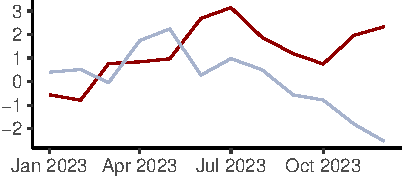
\includegraphics[keepaspectratio]{example_slides_files/figure-beamer/tsplot1-1.pdf}}

\vspace{-5pt}
\begin{minipage}{0.9\textwidth}
\scriptsize
\singlespacing
\textbf{Notes:} You can use this text to provide further information about the table. \lipsum[66]
\end{minipage}
\vspace{15pt}

}

\end{figure}%
\end{frame}

\begin{frame}{Scatterplot}
\phantomsection\label{scatterplot}
\begin{figure}

\caption{\label{fig-scatterplot}Two groups have very different values}

\centering{

\pandocbounded{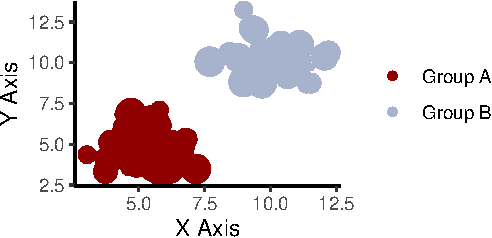
\includegraphics[keepaspectratio]{example_slides_files/figure-beamer/scatterplot-1.pdf}}

\vspace{-5pt}
\begin{minipage}{0.9\textwidth}
\scriptsize
\singlespacing
\textbf{Notes:} You can use this text to provide further information about the table. \lipsum[66]
\end{minipage}
\vspace{15pt}

}

\end{figure}%
\end{frame}

\begin{frame}{Dotplot}
\phantomsection\label{dotplot}
\begin{figure}

\caption{\label{fig-dotplot}Visualizing distributions with few
observations}

\centering{

\pandocbounded{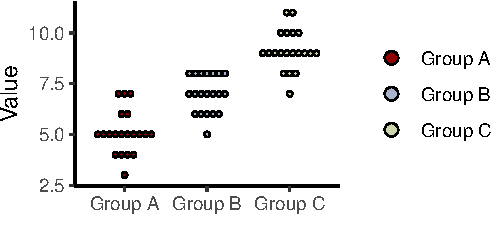
\includegraphics[keepaspectratio]{example_slides_files/figure-beamer/dotplot-1.pdf}}

\vspace{-10pt}
\begin{minipage}{0.9\textwidth}
\scriptsize
\singlespacing
\textbf{Notes:} You can use this text to provide further information about the table. \lipsum[66]
\end{minipage}
\vspace{15pt}

}

\end{figure}%
\end{frame}

\begin{frame}{Event Study}
\phantomsection\label{event-study}
\begin{figure}

\caption{\label{fig-eventstudy}Coefficients relative to treatment time}

\centering{

\pandocbounded{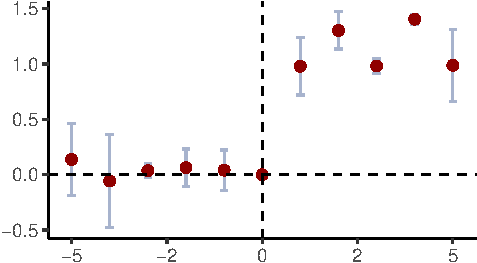
\includegraphics[keepaspectratio]{example_slides_files/figure-beamer/eventstudy-1.pdf}}

\vspace{-10pt}
\begin{minipage}{0.9\textwidth}
\scriptsize
\singlespacing
\textbf{Notes:} You can use this text to provide further information about the table. \lipsum[66]
\end{minipage}
\vspace{15pt}

}

\end{figure}%
\end{frame}

\begin{frame}{Tourism overnight stays in southern Germany in 2023}
\phantomsection\label{tourism-overnight-stays-in-southern-germany-in-2023}
\begin{figure}

\caption{\label{fig-choro}This is a choropleth map}

\centering{

\pandocbounded{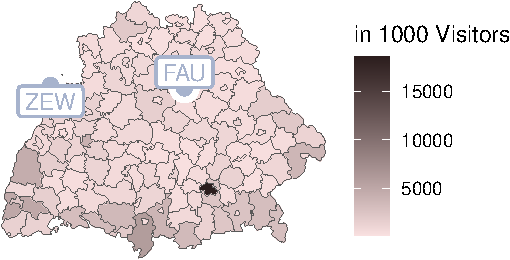
\includegraphics[keepaspectratio]{example_slides_files/figure-beamer/choro-1.pdf}}

\vspace{-10pt}
\begin{minipage}{0.9\textwidth}
\scriptsize
\singlespacing
\textbf{Notes:} You can use this text to provide further information about the table. \lipsum[66]
\end{minipage}
\vspace{15pt}

}

\end{figure}%
\end{frame}

\begin{frame}{Counties with University Hospitals in southern Germany in
2023}
\phantomsection\label{counties-with-university-hospitals-in-southern-germany-in-2023}
\begin{figure}

\caption{\label{fig-indic}This is an indicator map}

\centering{

\pandocbounded{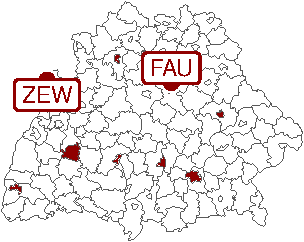
\includegraphics[keepaspectratio]{example_slides_files/figure-beamer/indic-1.pdf}}

\vspace{-10pt}
\begin{minipage}{0.9\textwidth}
\scriptsize
\singlespacing
\textbf{Notes:} You can use this text to provide further information about the table. \lipsum[66]
\end{minipage}
\vspace{15pt}

}

\end{figure}%
\end{frame}

\section{Tables}\label{tables}

\begin{frame}{Descriptives Table}
\phantomsection\label{descriptives-table}
\begin{table}

\caption{\label{tbl-descriptives}Descriptive statistics by group}

\centering{

\fontsize{12.0pt}{14.4pt}\selectfont
\begin{tabular*}{\linewidth}{@{\extracolsep{\fill}}lcc}
\toprule
\textbf{Characteristic} & \textbf{0}\\
N = 265 & \textbf{1}\\
N = 235 \\ 
\midrule\addlinespace[2.5pt]
Survival & 0.16 (0.37) & 0.47 (0.50) \\ 
Age in years & 49.86 (16.75) & 50.50 (17.93) \\ 
Female & 0.51 (0.50) & 0.52 (0.50) \\ 
Severity Score & 0.39 (0.49) & 0.36 (0.48) \\ 
\bottomrule
\end{tabular*}
\begin{minipage}{\linewidth}
­\\
\textbf{Notes:} Here is additional information
on the table, which can be lengthy. It does
not have to be but in order to check for line
breaks, it makes sense to have it this way.
It does not have to be but in order to check
for line breaks, it makes sense to have it
this way.\\
\end{minipage}

}

\end{table}%
\end{frame}

\begin{frame}{Regression Tables}
\phantomsection\label{regression-tables}
\begin{table}

\caption{\label{tbl-regression}Linear Regression Models}

\centering{

\fontsize{12.0pt}{14.4pt}\selectfont
\begin{tabular*}{\linewidth}{@{\extracolsep{\fill}}lcccccc}
\toprule
 & \multicolumn{2}{c}{Full Sample} & \multicolumn{2}{c}{Men} & \multicolumn{2}{c}{Women} \\ 
\cmidrule(lr){2-3} \cmidrule(lr){4-5} \cmidrule(lr){6-7}
  & (I) & (II) & (III) & (IV) & (V) & (VI) \\ 
\midrule\addlinespace[2.5pt]
Treatment & 0.310*** & 0.299*** & 0.337*** & 0.326*** & 0.284*** & 0.267*** \\ 
{} & {(0.040)} & {(0.038)} & {(0.057)} & {(0.053)} & {(0.055)} & {(0.054)} \\ 
N & 500 & 500 & 242 & 242 & 258 & 258 \\ 
R² & 0.11 & 0.20 & 0.13 & 0.25 & 0.10 & 0.17 \\ 
\bottomrule
\end{tabular*}
\begin{minipage}{\linewidth}
­\\
\textbf{Notes:} Here is additional information on the table, which can be
lengthy. It does not have to be but in order to check for line breaks,
it makes sense to have it this way. It does not have to be but in order
to check for line breaks, it makes sense to have it this way.\\
\end{minipage}

}

\end{table}%
\end{frame}

\section{What we have learned}\label{what-we-have-learned}

\begin{frame}{Last Slide}
\phantomsection\label{last-slide}
This slide will most likely be the one that the audience sees the
longest. Take this into account when designing it. We could for example
point out the following things:

\begin{itemize}
\tightlist
\item
  A literature slide can be at the end of your presentation, but not to
  show it while the audience is discussing your paper (ok, maybe if you
  conducted a literature review\ldots).
\item
  If you present a table and say: ``\emph{Oh, this is probably a bit
  small}'', then 1) you are probably right and 2) you could have changed
  it in advance.
\end{itemize}
\end{frame}

\section{Appendix}\label{appendix}

\begin{frame}{Regression in the Appendix}
\phantomsection\label{regression-in-the-appendix}
% Always keep this code if you want to use an appendix

\renewcommand{\thetable}{A.\arabic{table}}
\renewcommand{\thefigure}{A.\arabic{figure}}
\setcounter{table}{0}
\setcounter{figure}{0}

\begin{table}

\caption{\label{tbl-regression2}Linear Regression Models for the
Appendix}

\centering{

\fontsize{12.0pt}{14.4pt}\selectfont
\begin{tabular*}{\linewidth}{@{\extracolsep{\fill}}lcccccc}
\toprule
 & \multicolumn{2}{c}{Full Sample} & \multicolumn{2}{c}{Men} & \multicolumn{2}{c}{Women} \\ 
\cmidrule(lr){2-3} \cmidrule(lr){4-5} \cmidrule(lr){6-7}
  & (I) & (II) & (III) & (IV) & (V) & (VI) \\ 
\midrule\addlinespace[2.5pt]
Treatment & 0.310*** & 0.299*** & 0.337*** & 0.326*** & 0.284*** & 0.267*** \\ 
{} & {(0.040)} & {(0.038)} & {(0.057)} & {(0.053)} & {(0.055)} & {(0.054)} \\ 
N & 500 & 500 & 242 & 242 & 258 & 258 \\ 
R² & 0.11 & 0.20 & 0.13 & 0.25 & 0.10 & 0.17 \\ 
\bottomrule
\end{tabular*}
\begin{minipage}{\linewidth}
­\\
\textbf{Notes:} Here is additional information on the table, which can be
lengthy. It does not have to be but in order to check for line breaks,
it makes sense to have it this way. It does not have to be but in order
to check for line breaks, it makes sense to have it this way.\\
\end{minipage}

}

\end{table}%
\end{frame}

\begin{frame}{Figures in the Appendix}
\phantomsection\label{figures-in-the-appendix}
\begin{figure}

\caption{\label{fig-two}Complex figure with two parts}

\centering{

\begin{figure}[H]

\begin{minipage}{0.05\linewidth}
~\end{minipage}%
%
\begin{minipage}{0.35\linewidth}
\subcaption{\label{}Time Series}

\pandocbounded{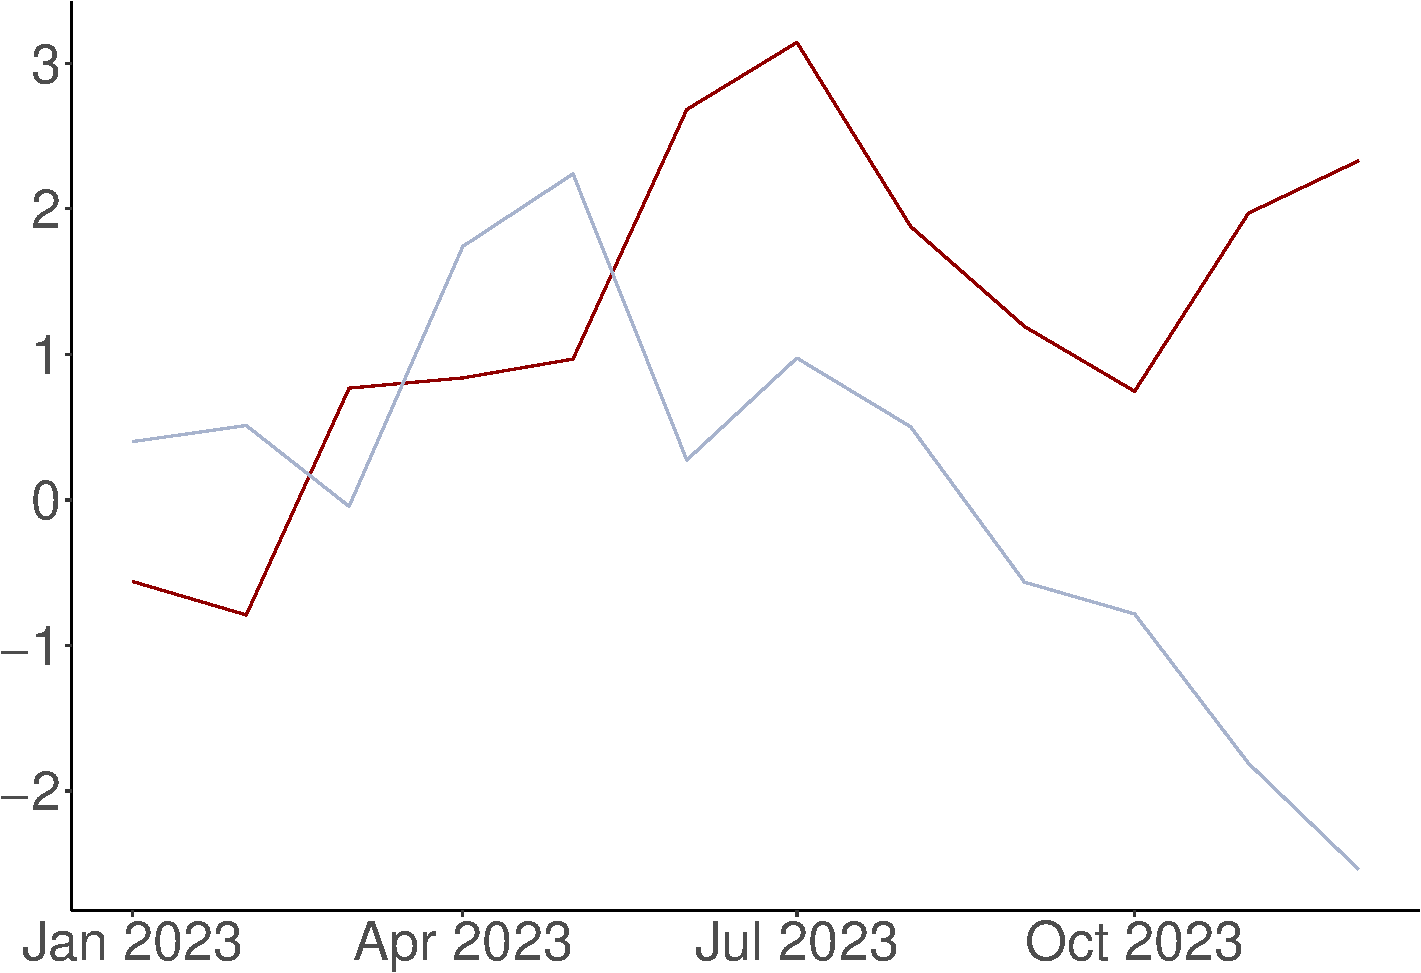
\includegraphics[keepaspectratio]{example_slides_files/figure-beamer/jointplot-1.pdf}}

\end{minipage}%
%
\begin{minipage}{0.20\linewidth}
~\end{minipage}%
%
\begin{minipage}{0.35\linewidth}
\subcaption{\label{}Scatterplot}

\pandocbounded{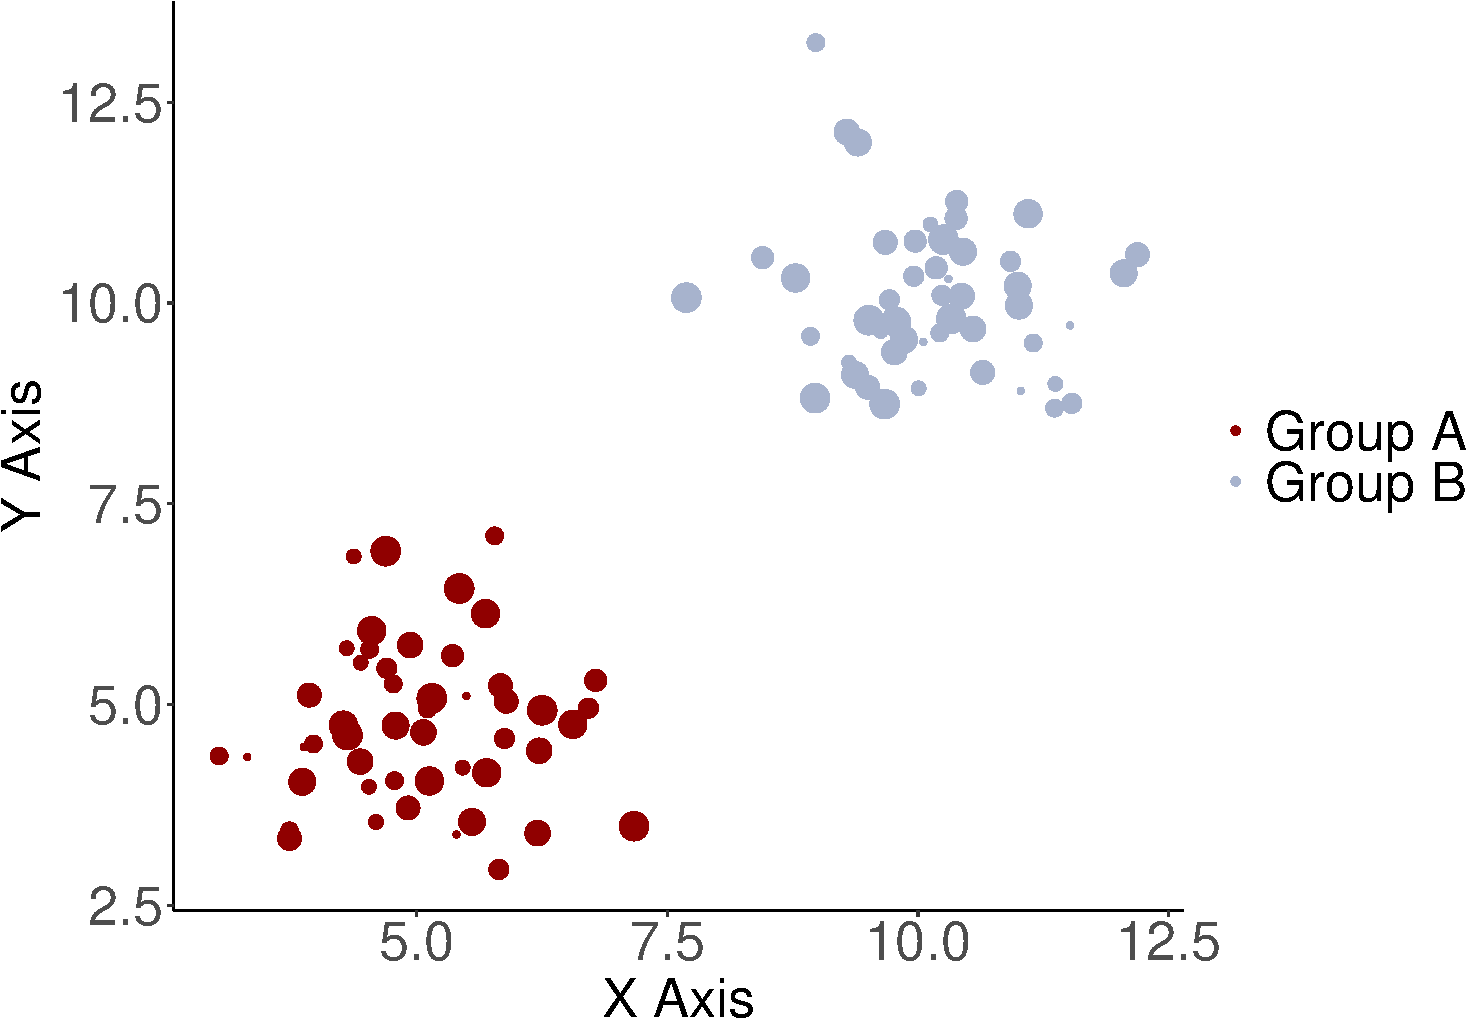
\includegraphics[keepaspectratio]{example_slides_files/figure-beamer/jointplot-2.pdf}}

\end{minipage}%
%
\begin{minipage}{0.05\linewidth}
~\end{minipage}%

\end{figure}%

\vspace{-5pt}
\begin{minipage}{0.9\textwidth}
\scriptsize
\singlespacing
\textbf{Notes:} You can use this text to provide further information about the table. \lipsum[66]
\end{minipage}
\vspace{15pt}

}

\end{figure}%
\end{frame}
\begin{frame}[allowframebreaks]{References}
\small
\printbibliography[heading=none]
\end{frame}
\end{document}
